\begin{figure}[H]
  \centering
  \textbf{Varying states }
  \newline
  \newline
  \pgfplotsset{
    scale only axis,
    legend style={at={(0,0.8)}, anchor=west, font=\tiny},
    xmin=7,
  }
  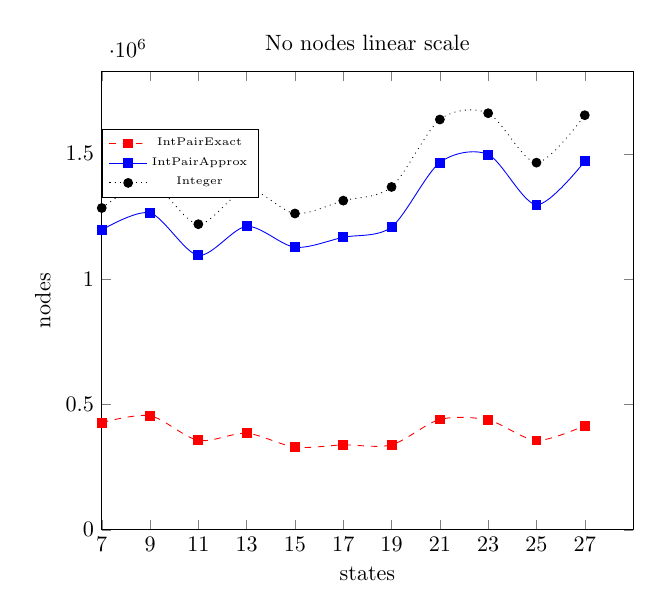
\begin{tikzpicture} [scale=0.8]
    \begin{axis}[
        title=No nodes linear scale,
        ylabel=nodes,
        xtick=data,
        ymin=0, 
        xlabel=states ]
      \addplot[smooth,mark=square*, mark options={solid},red, dashed]
      coordinates{ (7,427514) (9,454874) (11,356896) (13,385169) (15,329868) (17,338722) (19,339050) (21,440084) (23,437965) (25,356520) (27,415702)
      }; %\label{ie_plot}
      \addlegendentry{IntPairExact}
      \addplot[smooth,mark=square*, mark options={solid},blue]
      coordinates{ (7,1195984) (9,1264044) (11,1094910) (13,1210487) (15,1127178) (17,1166840) (19,1207856) (21,1464930) (23,1496955) (25,1296590) (27,1470000)
      }; %\label{ia_plot}
      \addlegendentry{IntPairApprox}
      \addplot[smooth,mark=*,mark options={solid},black, dotted]
      coordinates{ (7,1283617) (9,1382304) (11,1219058) (13,1358874) (15,1261790) (17,1313042) (19,1367570) (21,1636624) (23,1661830) (25,1464554) (27,1653812)
      }; %\label{int_plot}
      \addlegendentry{Integer}
    \end{axis}
  \end{tikzpicture}
  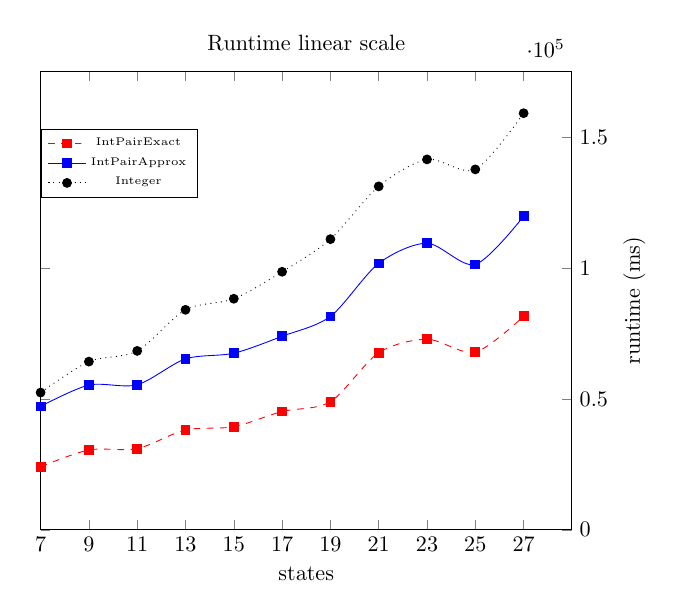
\begin{tikzpicture} [scale=0.8]
    \begin{axis}[
        yticklabel pos=right,
        xtick=data,
        title=Runtime linear scale,
        ylabel=runtime (ms),
        xlabel=states,
        ymin=0, ]
      \addplot[smooth,mark=square*,mark options={solid},red, dashed]
      coordinates{ (7, 24091) (9, 30492) (11, 31026) (13, 38125) (15, 39380) (17, 45187) (19, 48943) (21, 67630) (23, 72791) (25, 67855) (27, 81536)
      };% \label{IntPairExact Run}
      \addplot[smooth,mark=square*,mark options={solid},blue]
      coordinates{ (7, 47133) (9, 55287) (11, 55408) (13, 65274) (15, 67460) (17, 73920) (19, 81508) (21, 101759) (23, 109442) (25, 101353) (27, 119748)
      }; %\label{IntPairApprox Run}
      \addplot[smooth,mark=*,mark options={solid},black, dotted]
      coordinates{ (7, 52426) (9, 64242) (11, 68331) (13, 84028) (15, 88250) (17, 98554) (19, 111021) (21, 131160) (23, 141472) (25, 137661) (27, 159120)
      }; %\label{IntegerRun}
      \addlegendentry{IntPairExact}
      \addlegendentry{IntPairApprox}
      \addlegendentry{Integer}
    \end{axis}
  \end{tikzpicture}

%  \begin{tikzpicture}[scale=1.4]
%    \draw[very thick] (-4,0) -- (4,0);
%    \draw[draw=white] (-5,-0.2) -- (5,-0.2);
%  \end{tikzpicture}


%  \begin{tikzpicture} [scale=0.8]
%    \begin{semilogyaxis}[
%        title=No nodes logarithmic scale,
%        ylabel=nodes,
%        xtick=data,
%        ymin=0, 
%        xlabel=states ]
%     \addplot[smooth,mark=square*, mark options={solid},red, dashed]
%      coordinates{ (7,427514) (9,454874) (11,356896) (13,385169) (15,329868) (17,338722) (19,339050) (21,440084) (23,437965) (25,356520) (27,415702)
%      }; %\label{ie_plot}
%      \addlegendentry{IntPairExact}
%      \addplot[smooth,mark=square*, mark options={solid},blue]
%      coordinates{ (7,1195984) (9,1264044) (11,1094910) (13,1210487) (15,1127178) (17,1166840) (19,1207856) (21,1464930) (23,1496955) (25,1296590) (27,1470000)
%      }; %\label{ia_plot}
%      \addlegendentry{IntPairApprox}
%      \addplot[smooth,mark=*,mark options={solid},black, dotted]
%      coordinates{ (7,1283617) (9,1382304) (11,1219058) (13,1358874) (15,1261790) (17,1313042) (19,1367570) (21,1636624) (23,1661830) (25,1464554) (27,1653812)
%      }; %\label{int_plot}
%      \addlegendentry{Integer}

%    \end{semilogyaxis}
%  \end{tikzpicture}
%  \begin{tikzpicture} [scale=0.8]
%    \begin{semilogyaxis}[
%        title=Runtime logaritmhic scale,
%        yticklabel pos=right,
%        xtick=data,
%        ylabel=runtime (ms),
%        xlabel=states,
%        ymin=0,  ]
%      \addplot[smooth,mark=square*,mark options={solid},red, dashed]
%      coordinates{ (7, 24091) (9, 30492) (11, 31026) (13, 38125) (15, 39380) (17, 45187) (19, 48943) (21, 67630) (23, 72791) (25, 67855) (27, 81536)
%      }; %\label{IntPairExact Run}
%      \addplot[smooth,mark=square*,mark options={solid},blue]
%      coordinates{ (7, 47133) (9, 55287) (11, 55408) (13, 65274) (15, 67460) (17, 73920) (19, 81508) (21, 101759) (23, 109442) (25, 101353) (27, 119748)
%     }; %\label{IntPairApprox Run}
%      \addplot[smooth,mark=*,mark options={solid},black, dotted]
%      coordinates{ (7, 52426) (9, 64242) (11, 68331) (13, 84028) (15, 88250) (17, 98554) (19, 111021) (21, 131160) (23, 141472) (25, 137661) (27, 159120)
%      }; %\label{IntegerRun}
%      \addlegendentry{IntPairExact}
%      \addlegendentry{IntPairApprox}
%      \addlegendentry{Integer}
%    \end{semilogyaxis}
%  \end{tikzpicture}
 \caption{Varying the number of states. The other parameters are fixed. Size of alphabet=7, max cost per transition=15 and number of steps=7.}\label{fig:states}
\end{figure}
